\section{Experimentation details}
\subsection{Application of Convolutional Sparse Coding on MNIST}
In this section, we show the result of applying unsupervised Convolutional Sparse Coding (denoted as CSC) previously presented in MNIST dataset.\\
Here, it's useless to have more than $2* Signal\_size$ not represent the number of atoms but its represent the number of filters, and we need fewer filters than atoms in the traditional Sparse Coding. Arbitrationally, we chose 64 filters of (8 $\times$ 8), this is not recommended to use filters larger than (7$\times$7) for MNIST dataset  \cite{best-practices-for-convolutional-neural-networks-applied-to-visual-document-analysis} however in our case we want to get more discriminant filters, so using larger filters is the solution.\\

\begin{figure}[h]
 \centering
 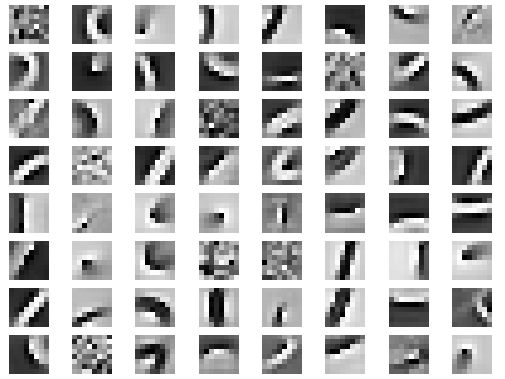
\includegraphics[scale=1]{CSC_D.png}
 % CSC_D.png: 640x480 px, 100dpi, 16.26x12.19 cm, bb=0 0 461 346
 \caption{Filters from the convolutional dictionary}
 \label{fig:CSC_D}
\end{figure}
As explained above,larger is the filter's size, more complex the pattern is. In our filters, we learned different types of curves (see figure \ref{fig:CSC_D}) that are more adapted to MNIST semantics. When we tried on smaller filter dimension we got  Gabor-like filters.\\
In order to use the activation maps obtained to make the classification, we want more complex models as possible. \\
In case of figure \ref{fig:CSC_D}, these curves are easy to find in some of our Latin/Western/Arabic numbers and are discriminative. For example, the second filter in figure \ref{fig:CSC_D} cannot be present for a handwritten 1.\\


\begin{figure}[h]
 \centering
 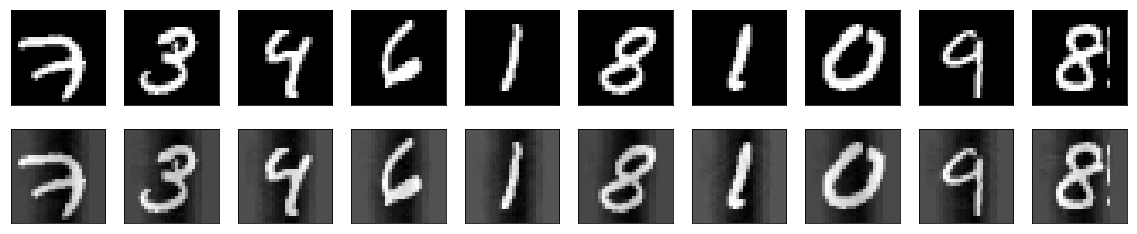
\includegraphics[scale=0.3]{CSC_reconstruction.png}
 % CSC_reconstruction.png: 1137x234 px, 72dpi, 40.12x8.26 cm, bb=0 0 1137 234
 \caption{Examples of reconstruction using CSC}
 \label{fig:CSC_recons}
\end{figure}

\begin{figure}[h]
 \centering
 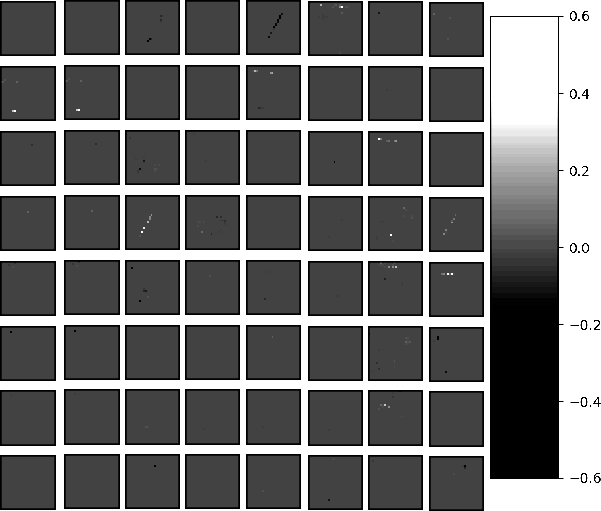
\includegraphics[scale=0.7]{MapActivation7.png}
 % MapActivation7.png: 601x511 px, 100dpi, 15.27x12.98 cm, bb=0 0 433 368
 \caption{Activation maps for a handwritten "7"}
 \label{fig:activationMaps}
\end{figure}

\begin{figure}[h]
 \centering
 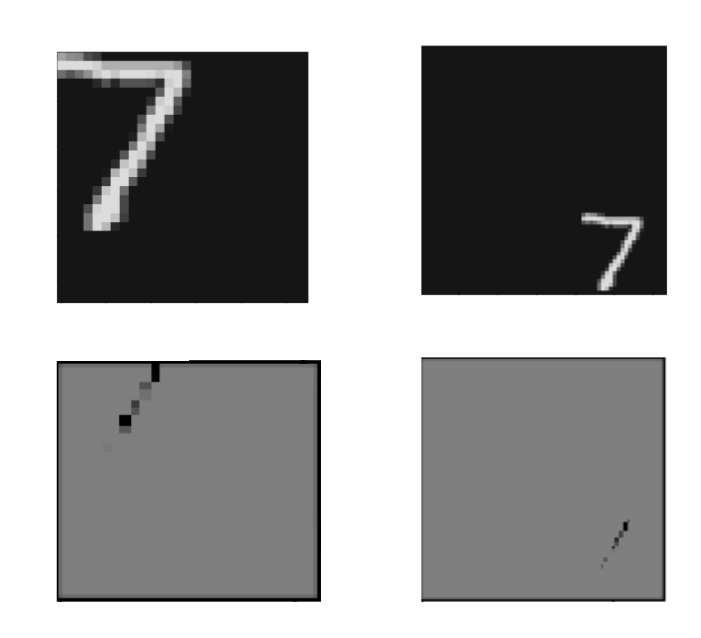
\includegraphics[scale=0.8]{CSC_Proof.png}
 % CSC_Proof.png: 701x638 px, 300dpi, 5.94x5.40 cm, bb=0 0 168 153
 \caption{Example of shift-invariance power in a characteristic features map ($5^{th}$ atom in the CSC dictionary)}
 \label{fig:CSCproof}
\end{figure}

As expected, Convolutional Sparse Coding detects the patterns in the input signal using the Sparse activation maps and the convolutional dictionary, which allows a good reconstruction(figure \ref{fig:CSC_recons}). But, as we can see in figure \ref{fig:activationMaps} and \ref{fig:CSCproof} in the activation maps, we obtained new patterns which are shift variant. Then we cannot apply the classification directly to these activation maps. To solve this problem, we tried different methods:
\begin{itemize}
 \item Max or Mean global pooling for each activation map:\\
 The objective was to create a unique activation card in which each pixel corresponds to the Max pooling of one of the 64 activation maps. But with these methods, we lose the pattern available in the activation maps, and consequently, discriminative pieces of information.
 \item Convolutional Sparse Coding on all activation maps:\\
 Apply on the activation maps a new convolutional sparse Coding. This method called Multi-Layer Convolutional Sparse Coding is described in the next chapter.
\end{itemize}
% 
% \newpage
% \subsection{Discussion}
% Using this examples we validate that CSC allow us to reconstruct our input data using filters, convolutions and activation maps. But we still cannot use activation maps for clustering or classification due to the non-discriminative reconstruction. Indeed, two seven in our test dataset haven't the same decomposition ( i.e. they don't have the same or close activation maps).
